% 2000 年广东卷第 5 题：函数 -x cos x 的四个图象选项
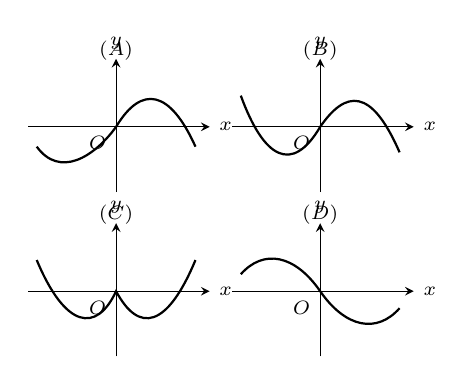
\begin{tikzpicture}[>=stealth, scale=0.72]
  \begin{scope}
    \node[font=\scriptsize] at (0,1.35) {$(A)$};
    \draw[->] (-1.55,0)--(1.65,0) node[right, font=\scriptsize] {$x$};
    \draw[->] (0,-1.15)--(0,1.2) node[above, font=\scriptsize] {$y$};
    \draw[thick] (-1.4,-0.35) .. controls (-1.0,-0.9) and (-0.4,-0.55) .. (0,0)
      .. controls (0.45,0.75) and (0.95,0.65) .. (1.4,-0.35);
    \node[below left, font=\scriptsize] at (0,0) {$O$};
  \end{scope}

  \begin{scope}[xshift=3.6cm]
    \node[font=\scriptsize] at (0,1.35) {$(B)$};
    \draw[->] (-1.55,0)--(1.65,0) node[right, font=\scriptsize] {$x$};
    \draw[->] (0,-1.15)--(0,1.2) node[above, font=\scriptsize] {$y$};
    \draw[thick] (-1.4,0.55) .. controls (-1.0,-0.55) and (-0.5,-0.85) .. (0,0)
      .. controls (0.45,0.65) and (0.9,0.7) .. (1.4,-0.45);
    \node[below left, font=\scriptsize] at (0,0) {$O$};
  \end{scope}

  \begin{scope}[yshift=-2.9cm]
    \node[font=\scriptsize] at (0,1.35) {$(C)$};
    \draw[->] (-1.55,0)--(1.65,0) node[right, font=\scriptsize] {$x$};
    \draw[->] (0,-1.15)--(0,1.2) node[above, font=\scriptsize] {$y$};
    \draw[thick] (-1.4,0.55) .. controls (-0.9,-0.65) and (-0.35,-0.75) .. (0,0)
      .. controls (0.4,-0.75) and (0.9,-0.65) .. (1.4,0.55);
    \node[below left, font=\scriptsize] at (0,0) {$O$};
  \end{scope}

  \begin{scope}[xshift=3.6cm,yshift=-2.9cm]
    \node[font=\scriptsize] at (0,1.35) {$(D)$};
    \draw[->] (-1.55,0)--(1.65,0) node[right, font=\scriptsize] {$x$};
    \draw[->] (0,-1.15)--(0,1.2) node[above, font=\scriptsize] {$y$};
    \draw[thick] (-1.4,0.3) .. controls (-1.0,0.75) and (-0.45,0.65) .. (0,0)
      .. controls (0.45,-0.65) and (1.0,-0.75) .. (1.4,-0.3);
    \node[below left, font=\scriptsize] at (0,0) {$O$};
  \end{scope}
\end{tikzpicture}
